\documentclass[a4paper,12pt]{article} % 设置字体大小为 12 点
\usepackage{fancyhdr}
\usepackage{listings}
\usepackage{xcolor}
\usepackage{hyperref}

\pagestyle{fancy}
\fancyhead[L]{Music and Methematics}
\fancyhead[R]{Spring 2024}

\renewcommand{\headrulewidth}{0.4pt} % 页眉下方的横线MLPDA
\renewcommand{\footrulewidth}{0pt} % 页脚下方的横线

% 将页眉线延伸到整个页面宽度
\fancyhfoffset[L]{0cm} % 左边距
\fancyhfoffset[R]{0cm} % 右边距
\headwidth=\textwidth

\usepackage{inputenc}
\usepackage[british,UKenglish]{babel}
\usepackage{amsmath}
%\usepackage{titlesec}
\usepackage{color}
\usepackage{graphicx}
\usepackage{fancyref}
\usepackage{hyperref}
\usepackage{float}
\usepackage{scrextend}
\usepackage{setspace}
\usepackage{xargs}
\usepackage{multicol}
\usepackage{nameref}

\usepackage{sectsty}
\usepackage{multicol}
\usepackage{multirow}
\usepackage[procnames]{listings}
\usepackage{appendix}
\usepackage{listings}

\newcommand\tab[1][1cm]{\hspace*{#1}}
\hypersetup{colorlinks=true, linkcolor=black}
\interfootnotelinepenalty=10000

\newcommand{\cleancode}[1]{\begin{addmargin}[3em]{3em}\texttt{\textcolor{cleanOrange}{#1}}\end{addmargin}}
\newcommand{\cleanstyle}[1]{\text{\textcolor{cleanOrange}{\texttt{#1}}}}


\usepackage[colorinlistoftodos,prependcaption,textsize=footnotesize]{todonotes}
\newcommandx{\commred}[2][1=]{\textcolor{Red}
{\todo[linecolor=red,backgroundcolor=red!25,bordercolor=red,#1]{#2}}}
\newcommandx{\commblue}[2][1=]{\textcolor{Blue}
{\todo[linecolor=blue,backgroundcolor=blue!25,bordercolor=blue,#1]{#2}}}
\newcommandx{\commgreen}[2][1=]{\textcolor{OliveGreen}{\todo[linecolor=OliveGreen,backgroundcolor=OliveGreen!25,bordercolor=OliveGreen,#1]{#2}}}
\newcommandx{\commpurp}[2][1=]{\textcolor{Plum}{\todo[linecolor=Plum,backgroundcolor=Plum!25,bordercolor=Plum,#1]{#2}}}

\def\code#1{{\tt #1}}

\def\note#1{\noindent{\bf [Note: #1]}}

\makeatletter
%% The "\@seccntformat" command is an auxiliary command
%% (see pp. 26f. of 'The LaTeX Companion,' 2nd. ed.)
\def\@seccntformat#1{\@ifundefined{#1@cntformat}%
   {\csname the#1\endcsname\quad}  % default
   {\csname #1@cntformat\endcsname}% enable individual control
}
\let\oldappendix\appendix %% save current definition of \appendix
\renewcommand\appendix{%
    \oldappendix
    \newcommand{\section@cntformat}{\appendixname~\thesection\quad}
}
\makeatother



\lstset{frame=, basicstyle={\footnotesize\ttfamily}}
\usepackage{geometry}
\geometry{left=3cm, right=3cm, top=4cm, bottom=3cm} % 设置页边距

\graphicspath{ {images/} }
\usepackage{ctex}
\usepackage{subcaption}
\usepackage{booktabs}
\usepackage[colorlinks,linkcolor=blue]{hyperref}
%-----------------------------------------BEGIN DOC----------------------------------------

\begin{document}
\renewcommand{\contentsname}{目\ 录}
\renewcommand{\appendixname}{附录}
\renewcommand{\appendixpagename}{附录}
\renewcommand{\refname}{参考文献} 
\renewcommand{\figurename}{图}
\renewcommand{\tablename}{表}
\renewcommand{\today}{\number\year 年 \number\month 月 \number\day 日}

\title{\textbf{{\Huge 音乐与数学选题四研究报告{\large\linebreak\\}}}\textbf{{\Large 噪声音乐 $\cdot$ 随机旋律的发展
 \linebreak\linebreak}}}
%please write your name, Student #, and Class # in Authors, student ID, and class # respectively
\author{ 
\\ 
\\
\\
\\
\\
组\ 长:\ 
张龄心\ \ 2100013018
\\组\ 员:\ 
邹灵萱\ \ 2100012868
\\ \ \ \ \ \ \ \ \ \ \ 冯之乐\ \ 2100012941
\\ \ \ \ \ \ \ \ \ \ \ 乔天硕\ \ 2100012999
\\ \ \ \ \ \ \ \ \ \ \ 赵亮然\ \ 2100013014
\\ 
\\
\\
\\
音乐与数学(春季, 2024)\\
北京大学\\
}
\date{\today}
\maketitle
\newpage

%-----------------------------------------CONTENT-------------------------------------
\begin{center}
\tableofcontents\label{c}
\end{center}
\newpage

%------------------------------------------TEXT--------------------------------------------

%----------------------------------------OVERVIEW-----------------------------------------

\section{音乐生成} \label{overview}%------------------------------
\subsection{概述}

本次大作业中,我们参考课堂内容和 Martin Gardner 的 Fractal Music, Hypercards and More,采用基于规则的方法生成随机音乐。我们选择音高和时值作为随机音乐的基本要素,使用 music21 库实现了白色、棕色、粉色音乐的生成器。我们将生成器的代码放在了 music\_gen/ 文件夹中,可以通过构造指定的生成器实例,生成任意长度、音域的音乐。

在介绍生成不同音乐的算法前,我们将生成的随机音乐抽象成音高和时值的序列,分别记为 $P_1, P_2, \ldots, P_n$ 和 $D_1, D_2, \ldots, D_n$。而随机音乐的生成算法,考虑的就是在已知 $(P_i, D_i)$ 的情况下,如何生成 $(P_{i+1}, D_{i+1})$。

\subsection{白色音乐的生成}

白色音乐是颜色音乐中相关性最低的一种。其中每一步的 $(P_{i+1}, D_{i+1})$ 都是独立生成,与 $(P_i, D_i)$ 无关。我们给出白色音乐的生成算法的伪代码:
\begin{lstlisting}[language=python]
function WhiteNoiseGen(N, PitchList, DurationList):
    P = []
    D = []
    for i = 1 to N:
        P.Append(Random(PitchList))
        D.Append(Random(DurationList))
    return P, D
\end{lstlisting}

\subsection{棕色音乐的生成}

棕色音乐是一种相关性较强的音乐。在生成 $(P_{i+1}, D_{i+1})$ 时,首先在给定范围内随机生成音高和时值的变化量,即 $\Delta P_i$ 和 $\Delta D_i$,然后计算

$$(P_{i+1}, D_{i+1}) = (P_i + \Delta P_i, D_i + \Delta D_i)$$

我们给出棕色音乐的生成算法的伪代码:
\begin{lstlisting}[language=python]
function BrownNoiseGen(N, StartPitch, StartDuration):
    P = [StartPitch]
    D = [StartDuration]
    for i = 2 to N:
        DeltaP = RandomPitchDelta(P[i-1])
        DeltaD = RandomDurationDelta(D[i-1])
        P.Append(P[i-1] + DeltaP)
        D.Append(D[i-1] + DeltaD)
    return P, D
\end{lstlisting}
值得一提的是,该算法并不要求当前处于不同的 $(P_i, D_i)$ 时,共享相同的变化量范围。因此当 $P_i$ 或 $D_i$ 已经到达边界时(可能是钢琴琴键的边界),我们可以通过改变变化量范围,保证 $(P_{i+1}, D_{i+1})$ 仍然在合法范围内。

最终,我们生成的棕色音乐的乐谱为:
\begin{figure}[H]
    \centering
    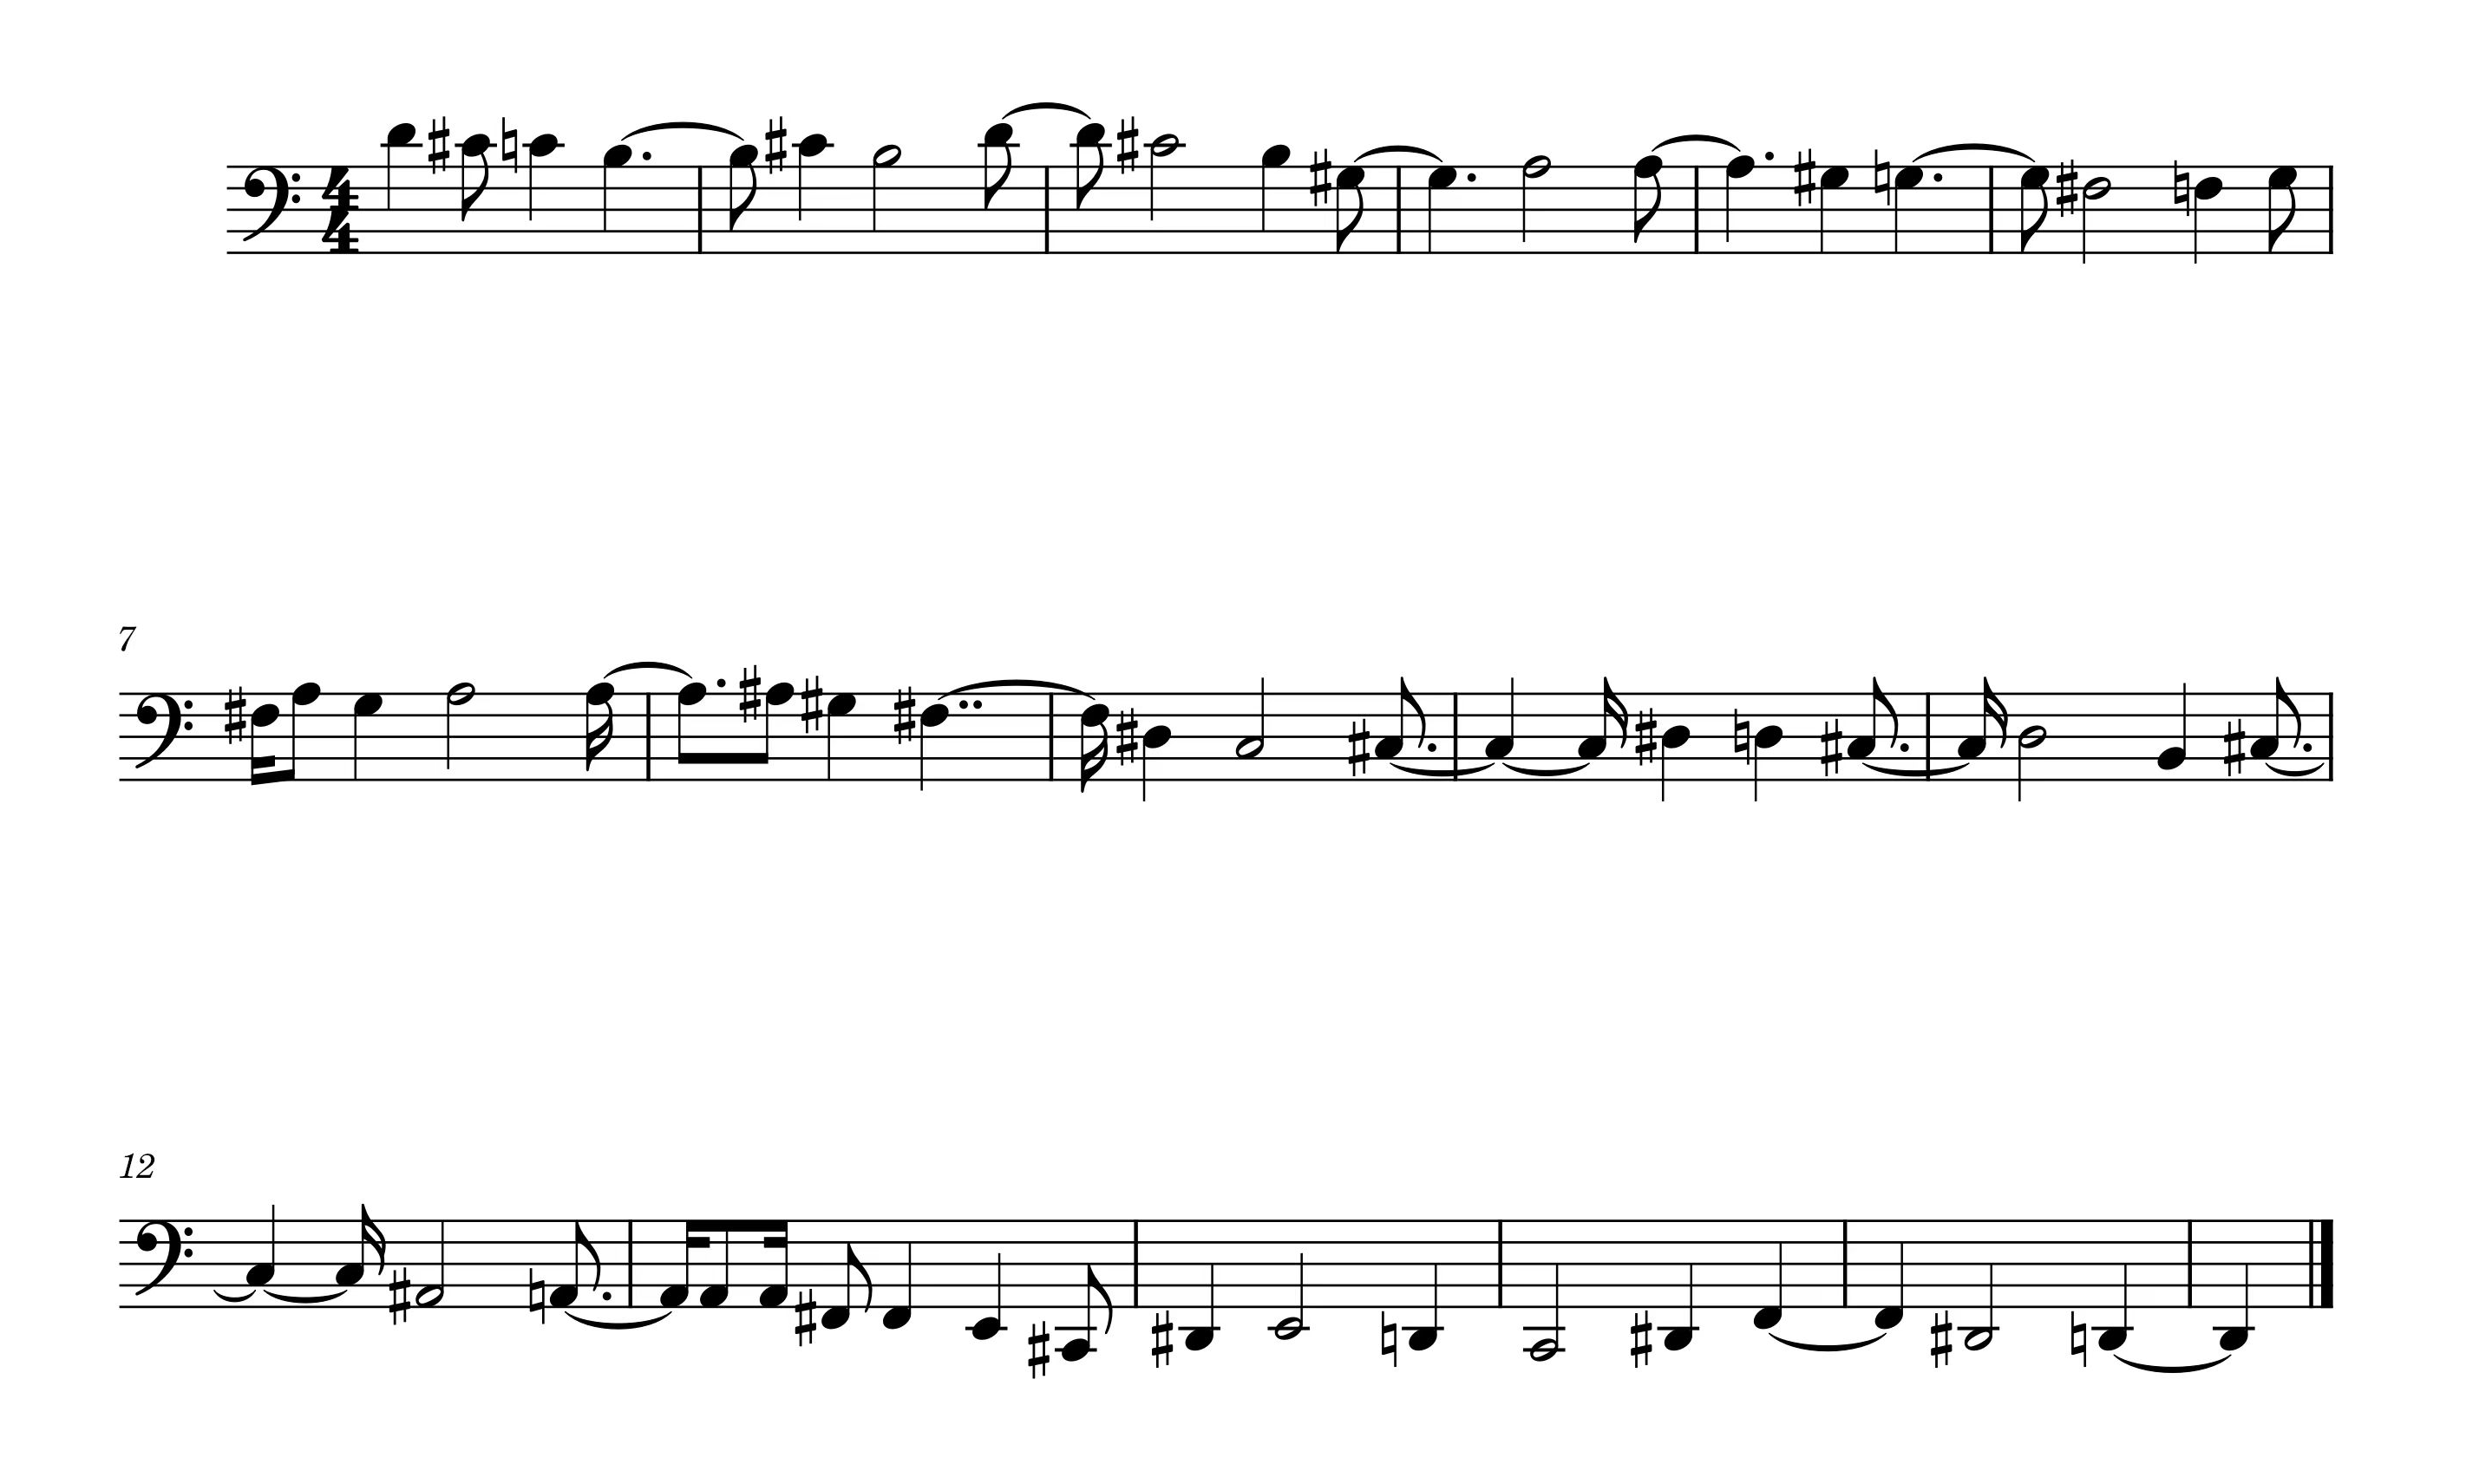
\includegraphics[width=1.0\linewidth]{images/brown.png}
    \caption{棕色音乐乐谱}
    \label{fig:enter-label}
\end{figure}

\subsection{粉色音乐的生成}

粉色音乐的相关性介于白色音乐和棕色音乐之间。关于粉色音乐的生成算法,我们以音高的生成为例。我们给出 $k$ 维向量 $Dice = (d_1, d_2, \ldots, d_k)$ ,其中 $d_i, i = 1, 2, \ldots, k$ 的取值范围是 $0, 1,\ldots, K$。在生成 $P_{i+1}$ 时,比较 $i$ 和 $i+1$ 在二进制表示下的每一位,如果不同,则重新选择 $Dice$ 这一分量的值,最终由 $Dice$ 各个分量的和决定 $P_{i+1}$。我们给出粉色音乐的生成算法的伪代码:
\begin{lstlisting}[language=python]
function PinkNoiseGen(N, PitchDice, DurationDice, PitchList, DurationList):
    P = [PitchList[Sum(PitchDice)]]
    D = [DurationList[Sum(DurationDice)]]
    for i = 2 to N:
        for j = 1 to k:
            if (GetBit(i, j) != GetBit(i-1, j)):
                PitchDice[j] = Random(K)
                DurationDice[j] = Random(K)
        P.Append(PitchList[Sum(PitchDice)])
        D.Append(DurationList[Sum(DurationDice)])
    return P, D
\end{lstlisting}

最终,我们生成的粉色音乐的乐谱为:
\begin{figure}[H]
    \centering
    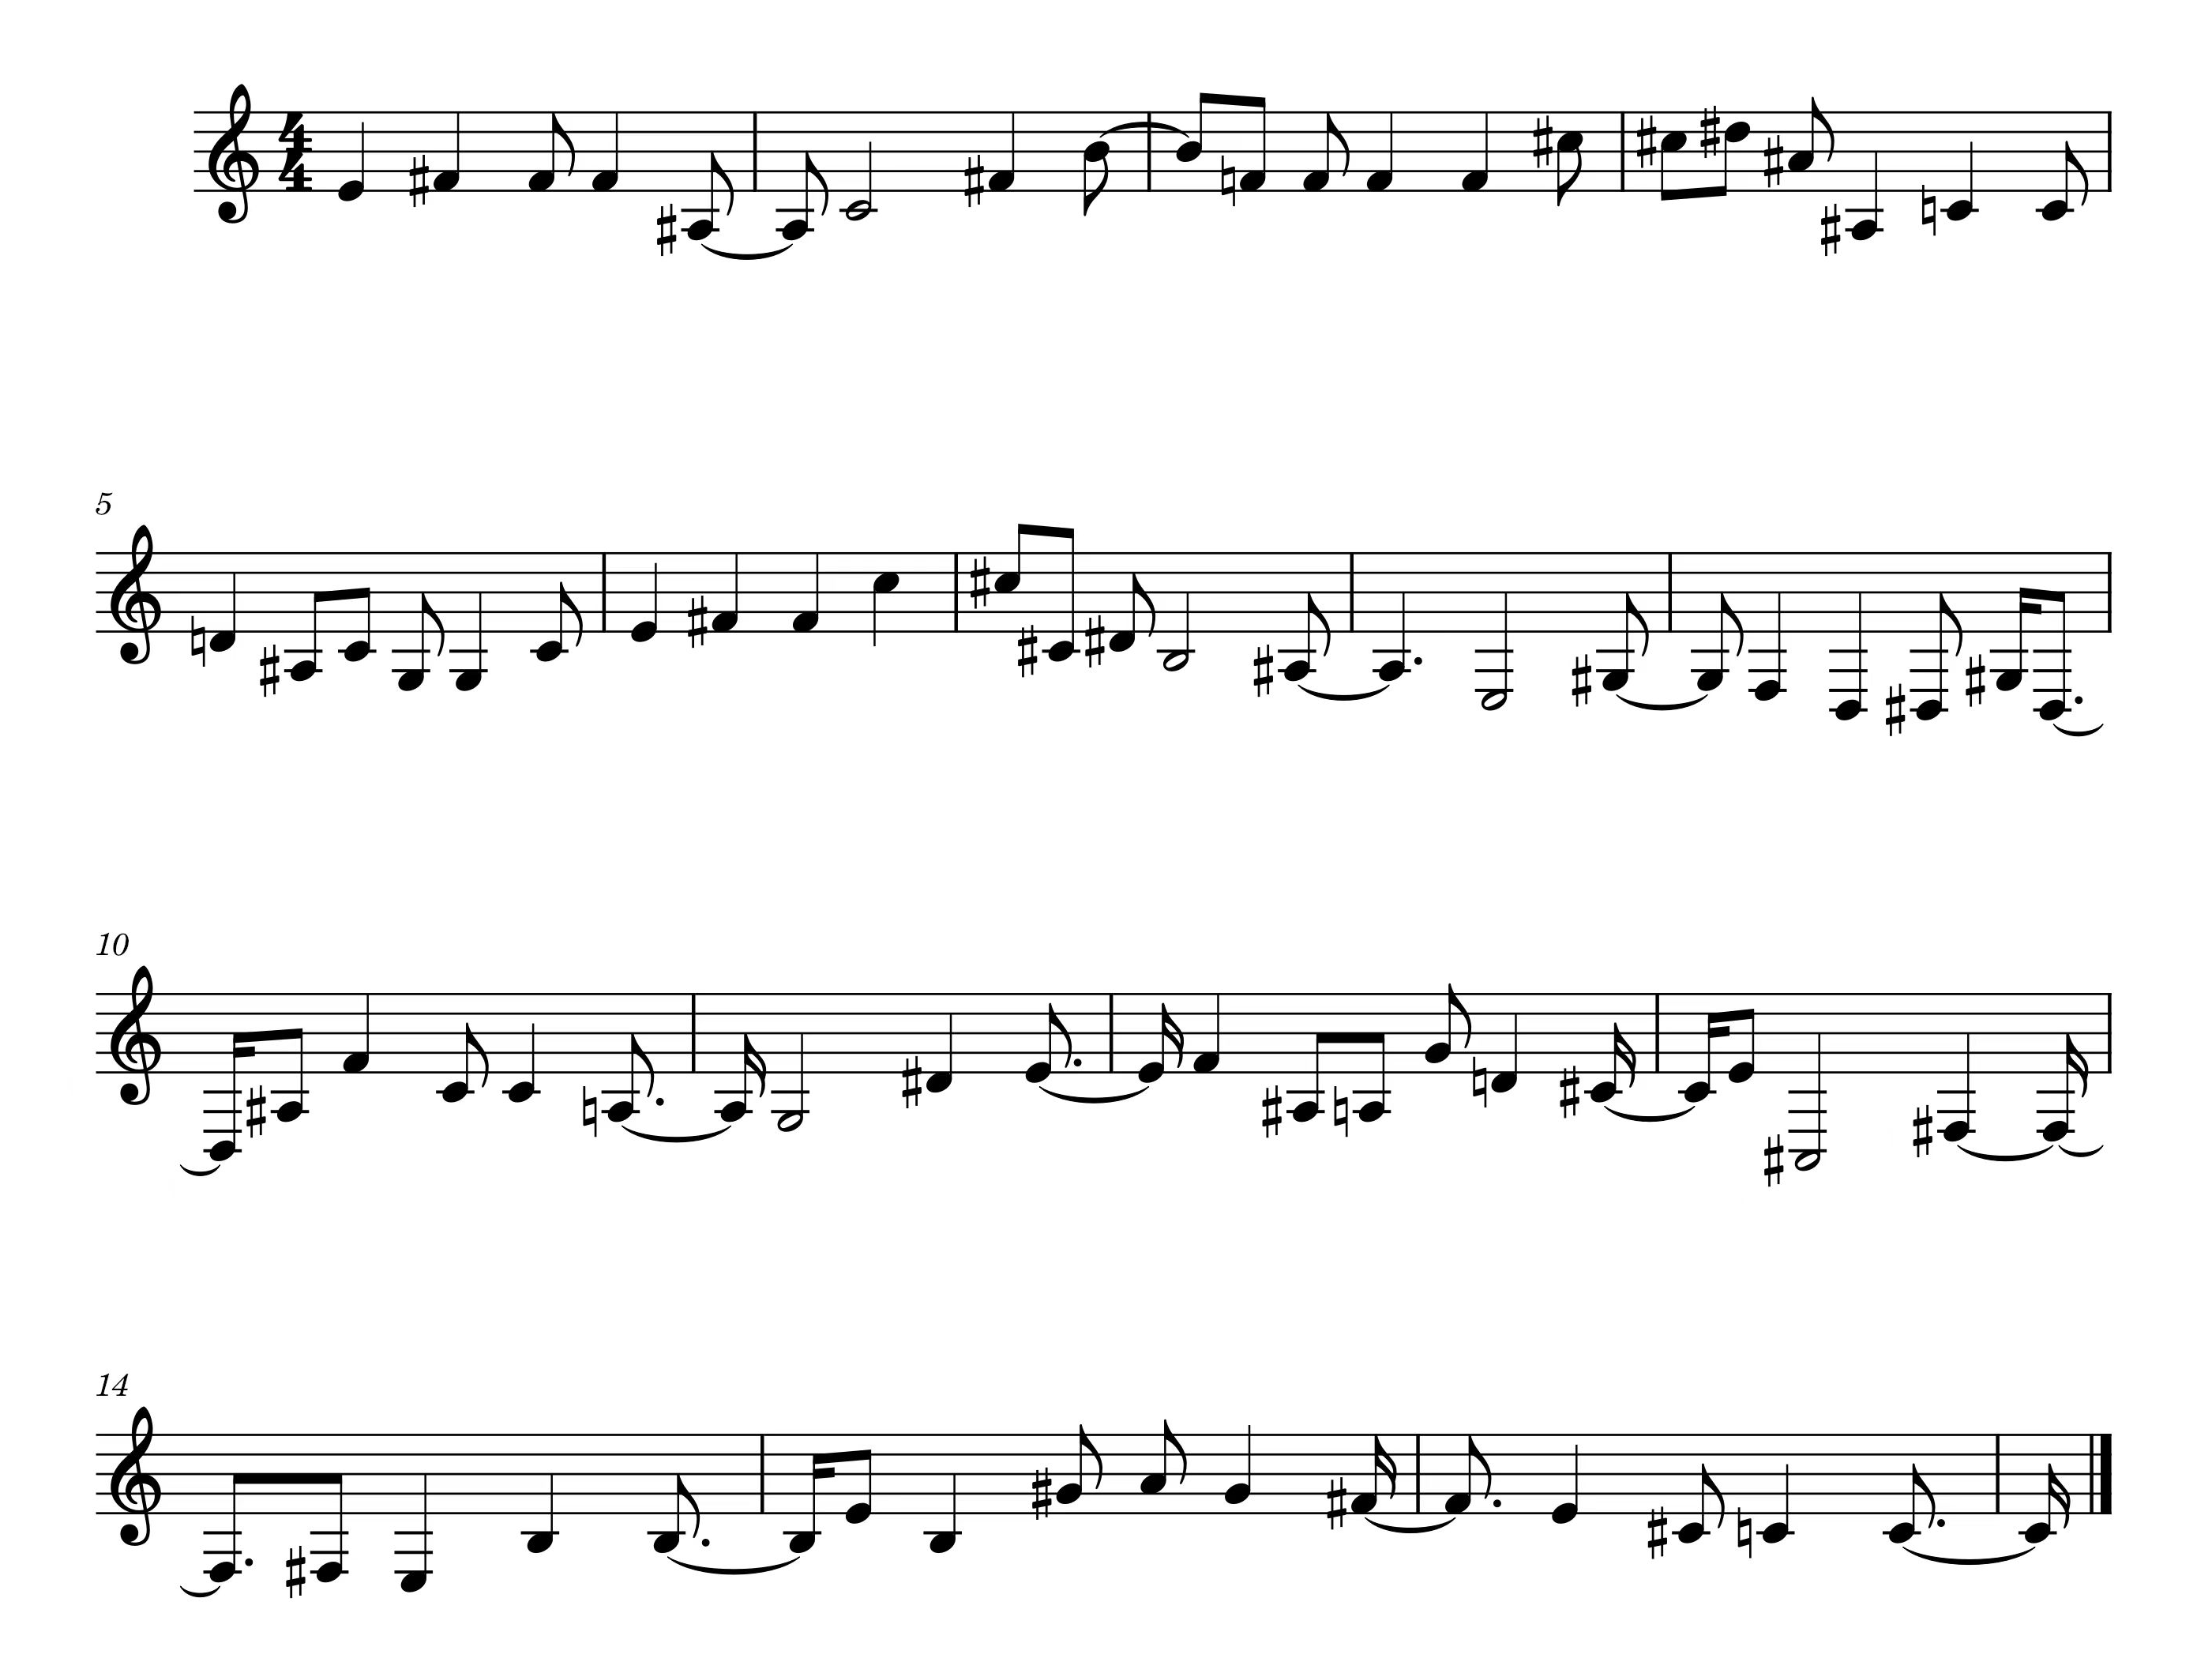
\includegraphics[width=1.0\linewidth]{images/pink.png}
    \caption{粉色音乐乐谱}
    \label{fig:enter-label}
\end{figure}

\subsection{总结}
该部分的工作主要是具体实现上述算法和基于已有的库(music21)构建音乐生成器。我们通过调整生成器的参数,生成了大量不同颜色、不同音域、不同长度的音乐,并通过比较这些音乐,感受到了白色、棕色、粉色音乐在相关性上的差异。

%------------------------------------Lab Process--------------------------------------
%------------------------------
\section{主观听感}
\subsection{棕色音乐}

\subsubsection{声音特质}
\begin{itemize}
    \item 曲调低:棕色噪声的低频成分多,高频成分较少,因而生成的这段音乐整体曲调较低,音调变化没有很大的跨度,集中在低音区。
\end{itemize}

\subsubsection{听觉体验}
\begin{itemize}
    \item 舒缓放松:由于低频成分多,较为舒缓柔和,没有压迫感和紧凑感,让人感到放松。
    \item 平稳:整体听起来平稳和持续,没有突然的变化,平和而不尖锐。
    \item 深沉:因为整体曲调较低,给人的感觉更深沉、更沉稳,类似于远处的雷声或海浪的声音。
\end{itemize}

\subsection{粉色音乐}

\subsubsection{声音特质}
\begin{itemize}
    \item 均衡感:粉色噪声在低频和高频之间具有更好的平衡,粉色音乐不尖锐也不低沉。
    \item 自然感:由于其频谱特性,粉色噪声生成的音乐虽然旋律感不强,但听起来较为自然。
\end{itemize}

\subsubsection{听觉体验}
\begin{itemize}
    \item 舒适和平滑:柔和平滑,没有突兀的音阶变化。
    \item 均匀和持续:乐声均匀和持续,提供一个较为稳定的听觉环境。
\end{itemize}

\subsection{两者对比}
棕色噪声的低频成分更为显著,因而棕色音乐听起来更为低沉和厚实,而粉色噪声则在低频和高频之间有更好的平衡,没有棕色噪声那么低沉,粉色音乐听起来更为柔和自然。

% --------------------------------Evaluation----------------------------------------
\section{乐谱分析}\label{ptxvsx86}
本章节将对粉色音乐和棕色音乐的乐谱进行自相关分析。\par
\subsection{自相关函数}
    自相关函数(ACF,Auto Correlation Function)是描述随机信号在不同时刻之间的相关程度的函数。\par
    对于连续信号$x(t)$,自相关函数定义为$$R_x(\tau)=\int_{-\infty}^{\infty}x(t)x(t+\tau)dt$$\par
    其中,$R_x(\tau)$反映信号在$t$时刻的取值与信号在$t-\tau$时刻取值的相关性。
    对于离散信号$x(n)$,其自相关函数定义为$$R_x(m)=\sum_{n=-\infty}^{\infty}x(n)x(n+m)$$\par
    其中,$R_x(m)$反映信号在$n$时刻的取值与信号在$n-m$时刻取值的相关性。\par
    对于大多数非周期性的时间序列,$R_x(m)$在m=0时的取值最大(时间序列与自身的相关程度最高)。而在m>0时,自相关函数会呈现下降趋势。减小速率越慢,则表明该时间序列的的自相关程度越高。\par
    Matlab软件中的autocorr函数可以求时间序列的自相关函数,并对函数进行归一化处理。在接下来的章节中,我们将利用Matlab对前文生的粉色音乐和棕色音乐的音高序列进行自相关分析。\par
\subsection{粉色音乐和棕色音乐的自相关分析}
    对于棕色音乐,我们设$C_3$对应的音高为1。每增高一个半音,音高加1;每减小一个,音高减1。按照以上规则,我们提取出来的棕色音乐音高序列为$$brown=[15\ 14\ 13\ 12\ ...\ -8\ -6\ -8\ -9]$$\par
    对于粉色音乐,我们$C_4$设对应的音高为1。每增高一个半音,音高加1;每减小一个半音,音高减1。最后提取出来的音高序列为$$pink=[5\ 7\ 11\ 1\ ...\ 7\ 5\ 2\ 1]$$\par
    提取完乐谱信息后,我们用Matlab的autocorr指令求时间序列brown和pink的自相关函数,并将它们绘制在同一张图中。Matlab代码如下所示。\par

\lstset{
  language=Matlab,  %代码语言使用的是matlab
  frame=single, %把代码用带有阴影的框圈起来
  commentstyle=\color{red!10!green!70}\textit,    % 设置代码注释的颜色
  showstringspaces=false,%不显示代码字符串中间的空格标记
  numbers=left, % 显示行号
  numberstyle=\tiny,    % 行号字体
  stringstyle=\ttfamily, % 代码字符串的特殊格式
  breaklines=true, %对过长的代码自动换行
  extendedchars=false,  %解决代码跨页时,章节标题,页眉等汉字不显示的问题
  texcl=true}
\begin{lstlisting}
%求自相关函数
brown = table2array(brown);
brown = brown';
ACF_brown = autocorr(brown);
pink = table2array(pink);
pink = pink';
ACF_pink = autocorr(pink);

%绘制曲线
t = 0:length(ACF_pink) - 1;
figure(1);
plot(t,abs(ACF_pink),'r');
hold on;
plot(t,abs(ACF_brown),'b');
xlabel('time');
ylabel('ACF');
legend('ACF\_pink','ACF\_brown');
title('粉色音乐和棕色音乐的自相关函数');
\end{lstlisting}
    最终绘制的brown和pink序列的自相关函数(ACF)曲线如下图所示。\par
\begin{figure}[htp]
\centering
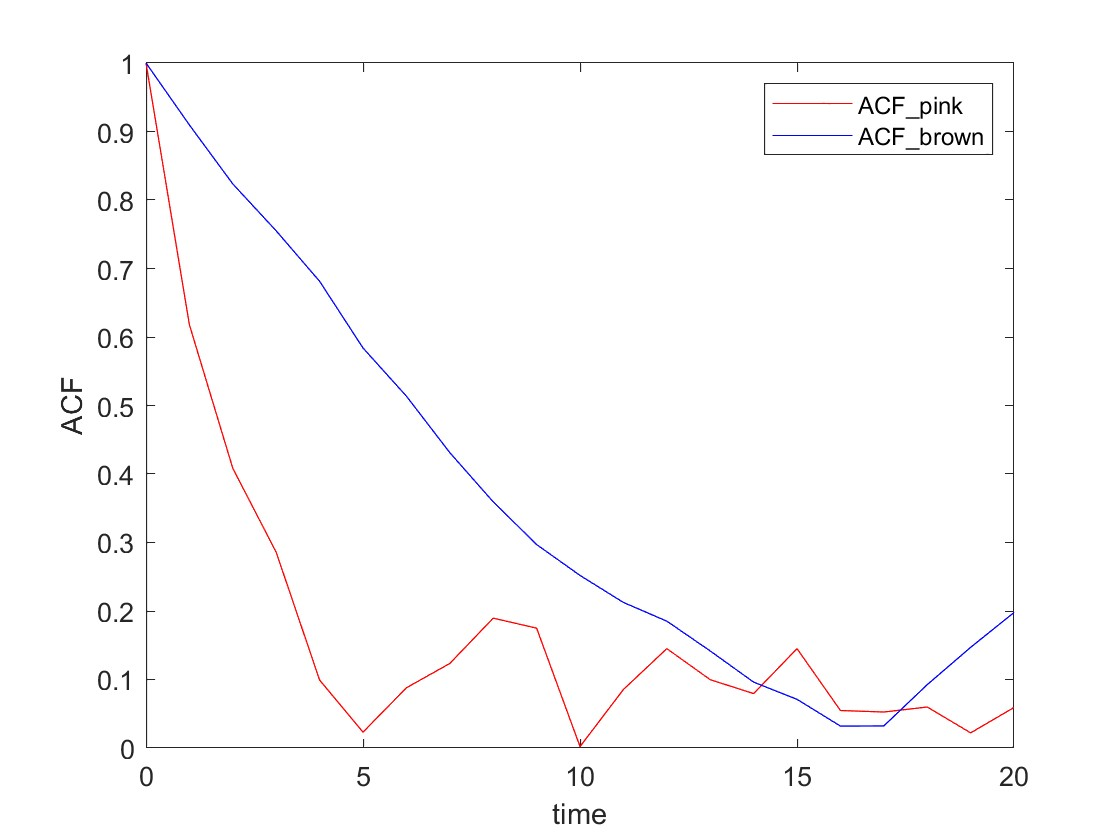
\includegraphics[width=0.8\linewidth]{ACF1.jpg}
\caption{粉色音乐和棕色音乐的自相关函数}
\label{}
\end{figure}
   通过对比我们可以发现,棕色音乐的自相关函数下降速率明显慢于粉色音乐。也就是说,棕色音乐具有更强的自相关性。这与实际情况相符合,从一定程度上证明了我们生成棕色音乐和粉色音乐方法的合理性。 \par

\section{编曲}\label{ptxvsx86}
\subsection{编曲方式的选择}
由于未对编曲的具体方式进行限制,一开始考虑过使用AI模型进行乐曲生成,例如Suno AI、Google的MusicFX、Meta开源的MusicGen等。

但调研后发现,Suno AI和MusicFX仅支持根据歌词和风格生成完整乐曲,无法自主选择旋律;MusicGen允许用户上传一段参考音频,但只是将参考音频融入生成的音乐中,并非以指定旋律为基础来生成音乐。

其他的AI音乐生成模型也有类似的问题,因此不符合我们的需要。

经过对比,还是选择了使用传统的编曲工具,也就是音频工作站(DAW)。

\subsection{基于棕色随机音乐的编曲}
\subsubsection{主旋律}
我从棕色音乐片段中选择了开头的四个小节:
\begin{figure}[H]
    \centering
    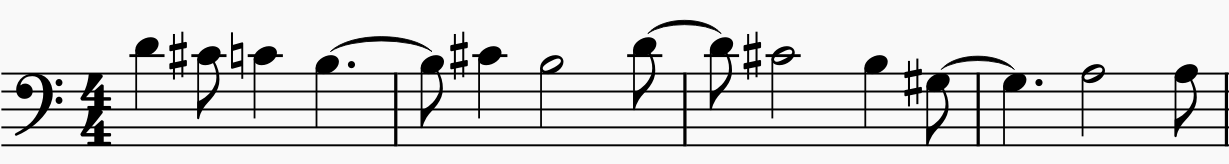
\includegraphics[width=0.8\linewidth]{images/Brown-motive-1.png}
    \caption{棕色音乐, 前4小节}
\end{figure}

更具体地,我选择了中间的这一小段旋律:

\begin{figure}[H]
    \centering
    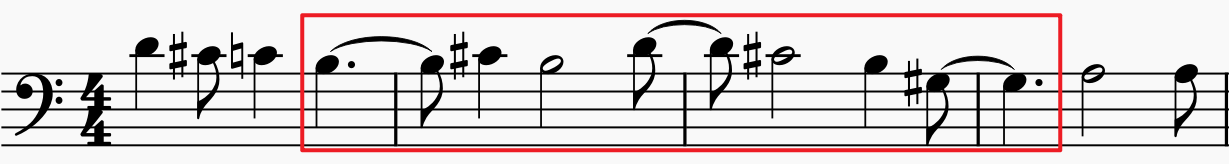
\includegraphics[width=0.8\linewidth]{images/Brown-motive-2.png}
    \caption{棕色音乐,前4小节,动机}
\end{figure}

由于音乐片段为随机生成,为了改善听感,也为了方便编曲,我对这个片段中音符的时值进行了改编。现在,这个旋律恰好能够放入两个4/4拍小节中:

\begin{figure}[H]
    \centering
    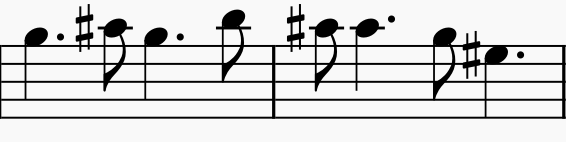
\includegraphics[width=0.4\linewidth]{images/Brown-motive-3.png}
    \caption{动机}
    \label{fig:brown-motive}
\end{figure}

移调,加入一些变奏,得到主旋律:

\begin{figure}[H]
    \centering
    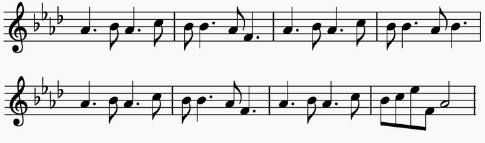
\includegraphics[width=0.8\linewidth]{images/Brown-main.png}
    \caption{主旋律(降A大调)}
    \label{fig:brown-main}
\end{figure}

\subsubsection{编曲结构}
音乐的主体是由上面的主旋律重复循环构成的,如图所示。

全曲长度约一分钟。
\begin{figure}[H]
    \centering
    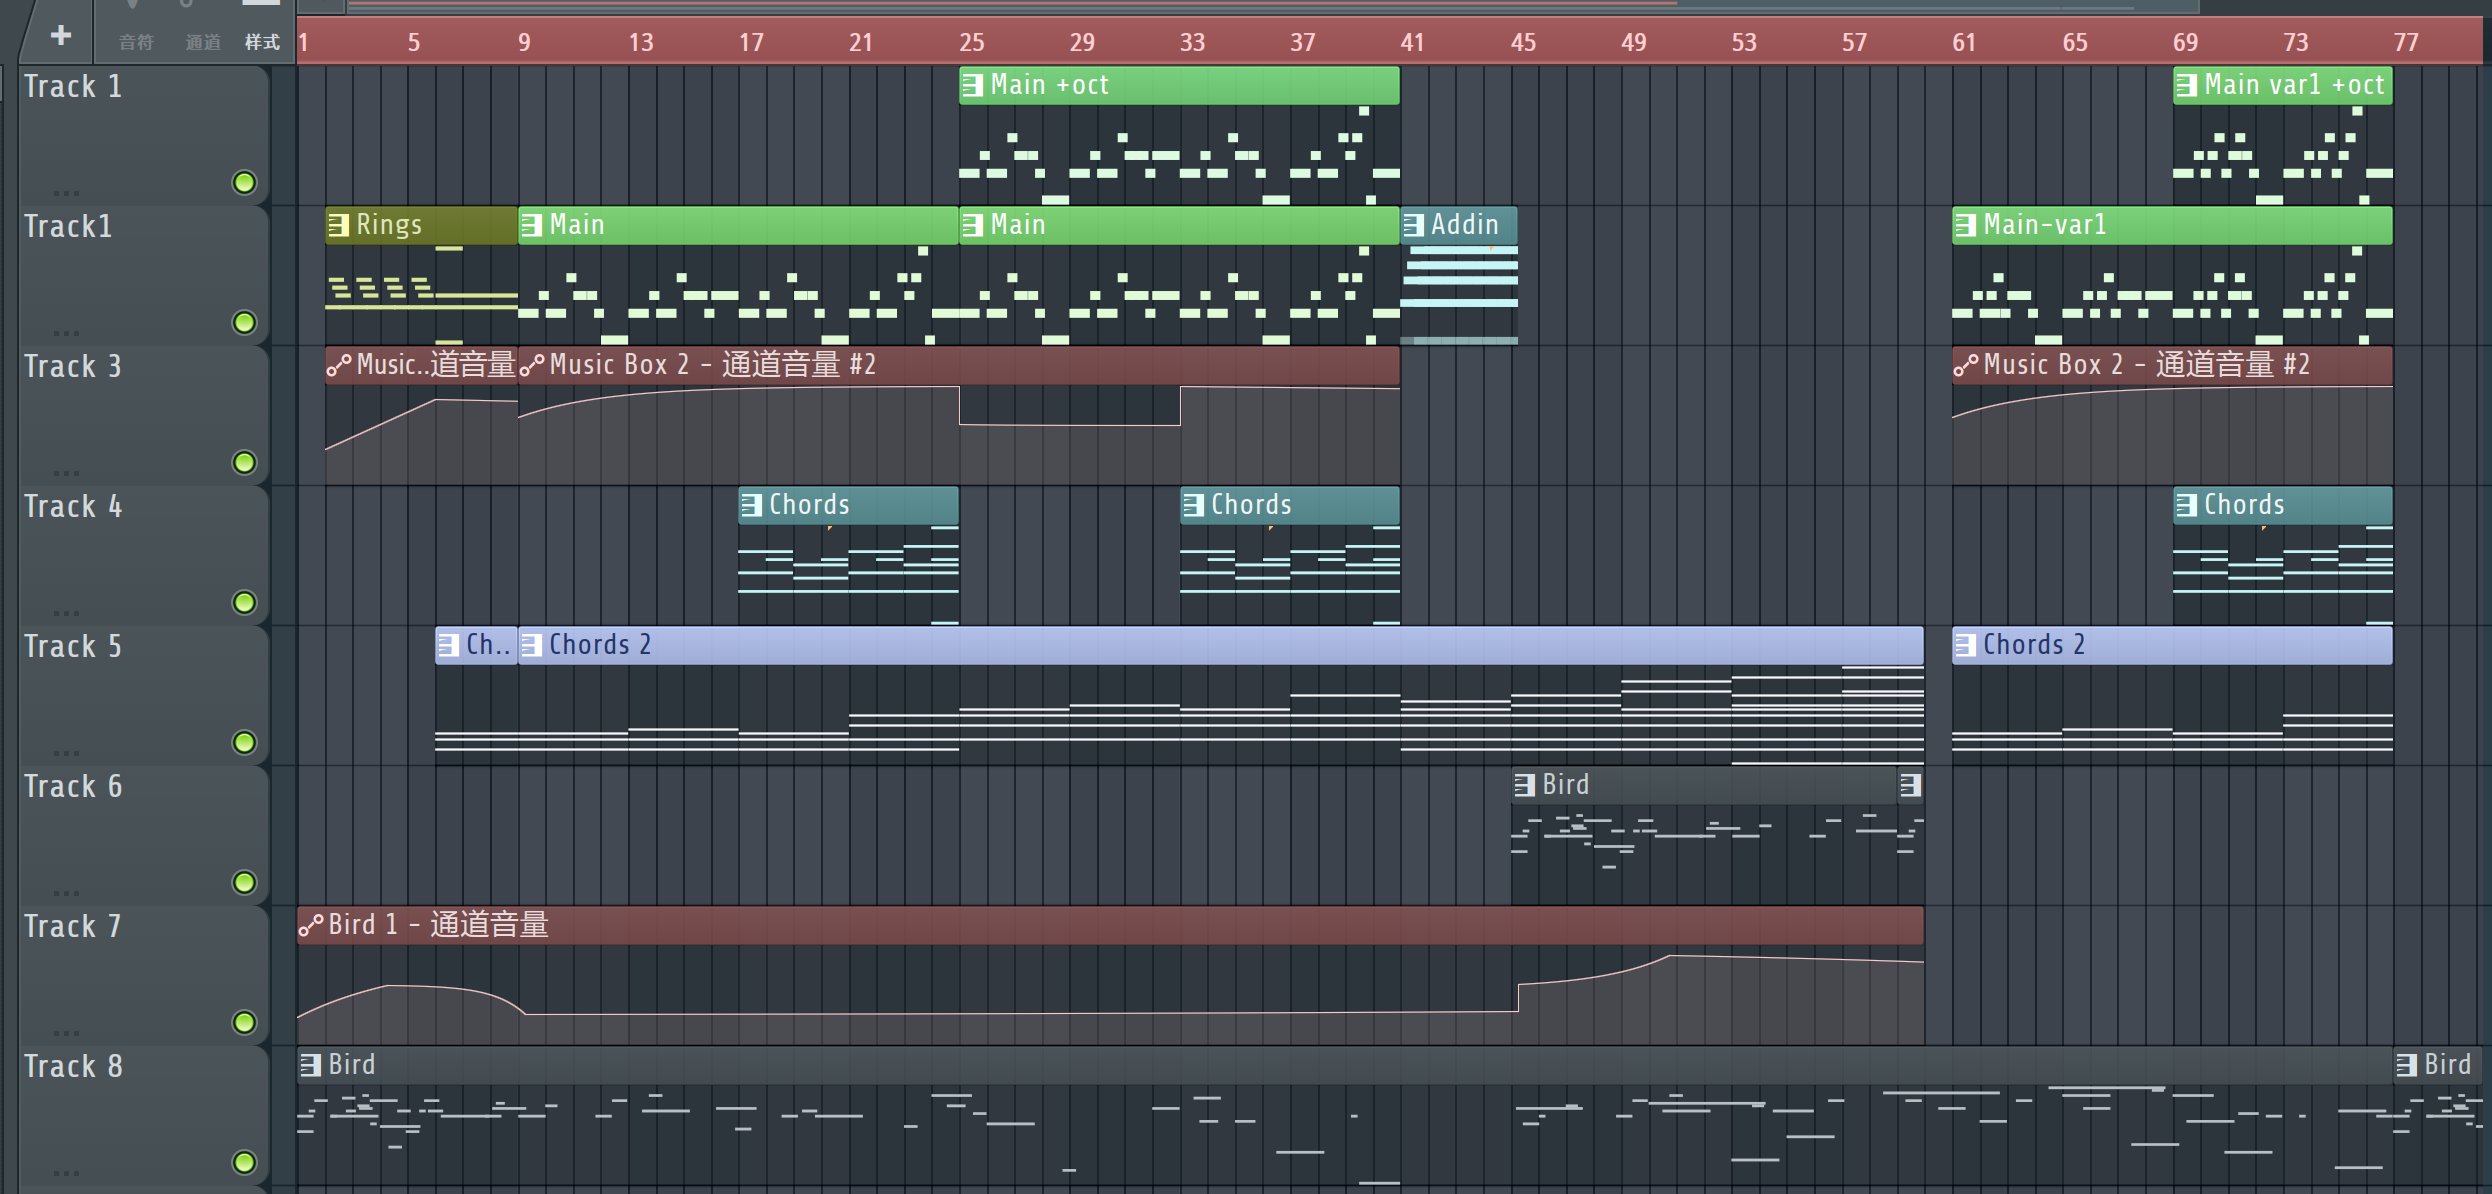
\includegraphics[width=1.0\linewidth]{images/Brown-flstudio.png}
    \caption{编曲结构}
    \label{fig:enter-label}
\end{figure}
\begin{itemize}
    \item 前奏:铃声以及明显的鸟鸣声,渐强。
    \item 第一部分:在前奏之后进入第一部分,主旋律重复两遍(渐强),以一段重复的短琶音结束。
    \item 第二部分:实际上是一段留白。之前作为背景音的和弦与鸟鸣声成为主角,主要能听到的是和弦的变化。
    \item 第三部分:重复第一部分的旋律,但加入变奏,同时音色也做出了一定调整。
    \item 尾声:以渐弱的鸟鸣声结束。
\end{itemize}


\subsubsection{乐器和音色}

我希望呈现一种比较轻灵的效果,因此为主旋律选择了类似八音盒的音色(FLEX - Music Box)。在旋律的几次重复中,我逐渐加入了钢琴、人声吟唱的合奏,使之显得更有层次感。

为了丰富听感,全曲加入了和弦(FLEX - Haunting Hour)和鸟鸣作为背景音。


\subsection{基于粉色随机音乐的编曲}
\subsubsection{主旋律}
我从粉色音乐片段中选择了结尾的三个小节:
\begin{figure}[H]
    \centering
    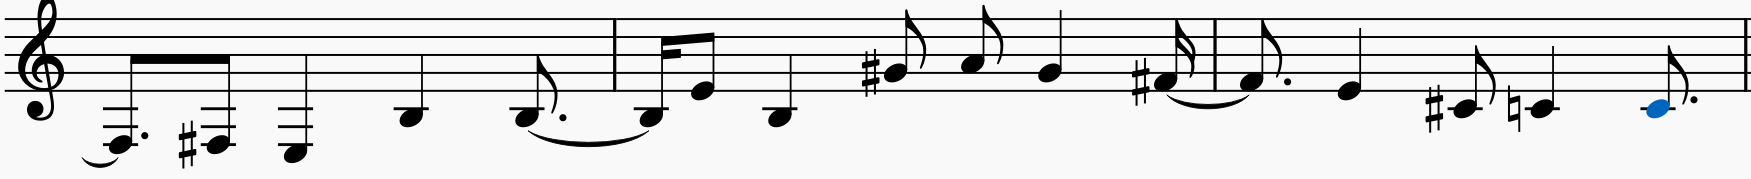
\includegraphics[width=0.8\linewidth]{images/Pink-motive-1.png}
    \caption{粉色音乐,后3小节}
    \label{fig:enter-label}
\end{figure}

采取中间这个旋律作为动机:
\begin{figure}[H]
    \centering
    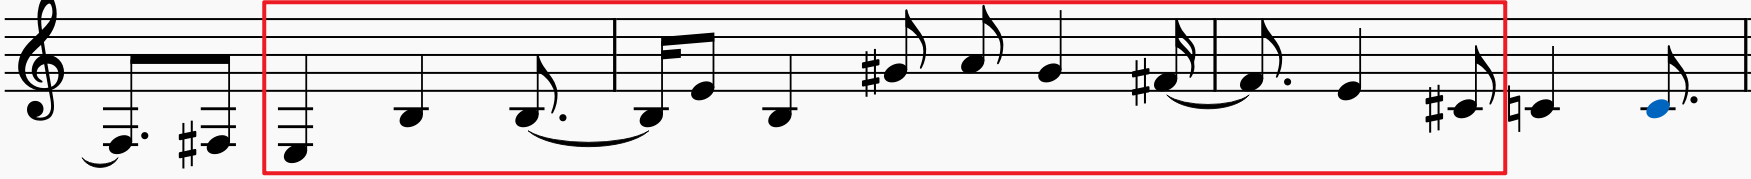
\includegraphics[width=0.8\linewidth]{images/Pink-motive-2.png}
    \caption{粉色音乐,后3小节,动机}
    \label{fig:enter-label}
\end{figure}

高八度,并加入一些变奏,得到下列片段,作为主旋律(主要部分恰好可以放入4个3/4拍的小节中):
\begin{figure}[H]
    \centering
    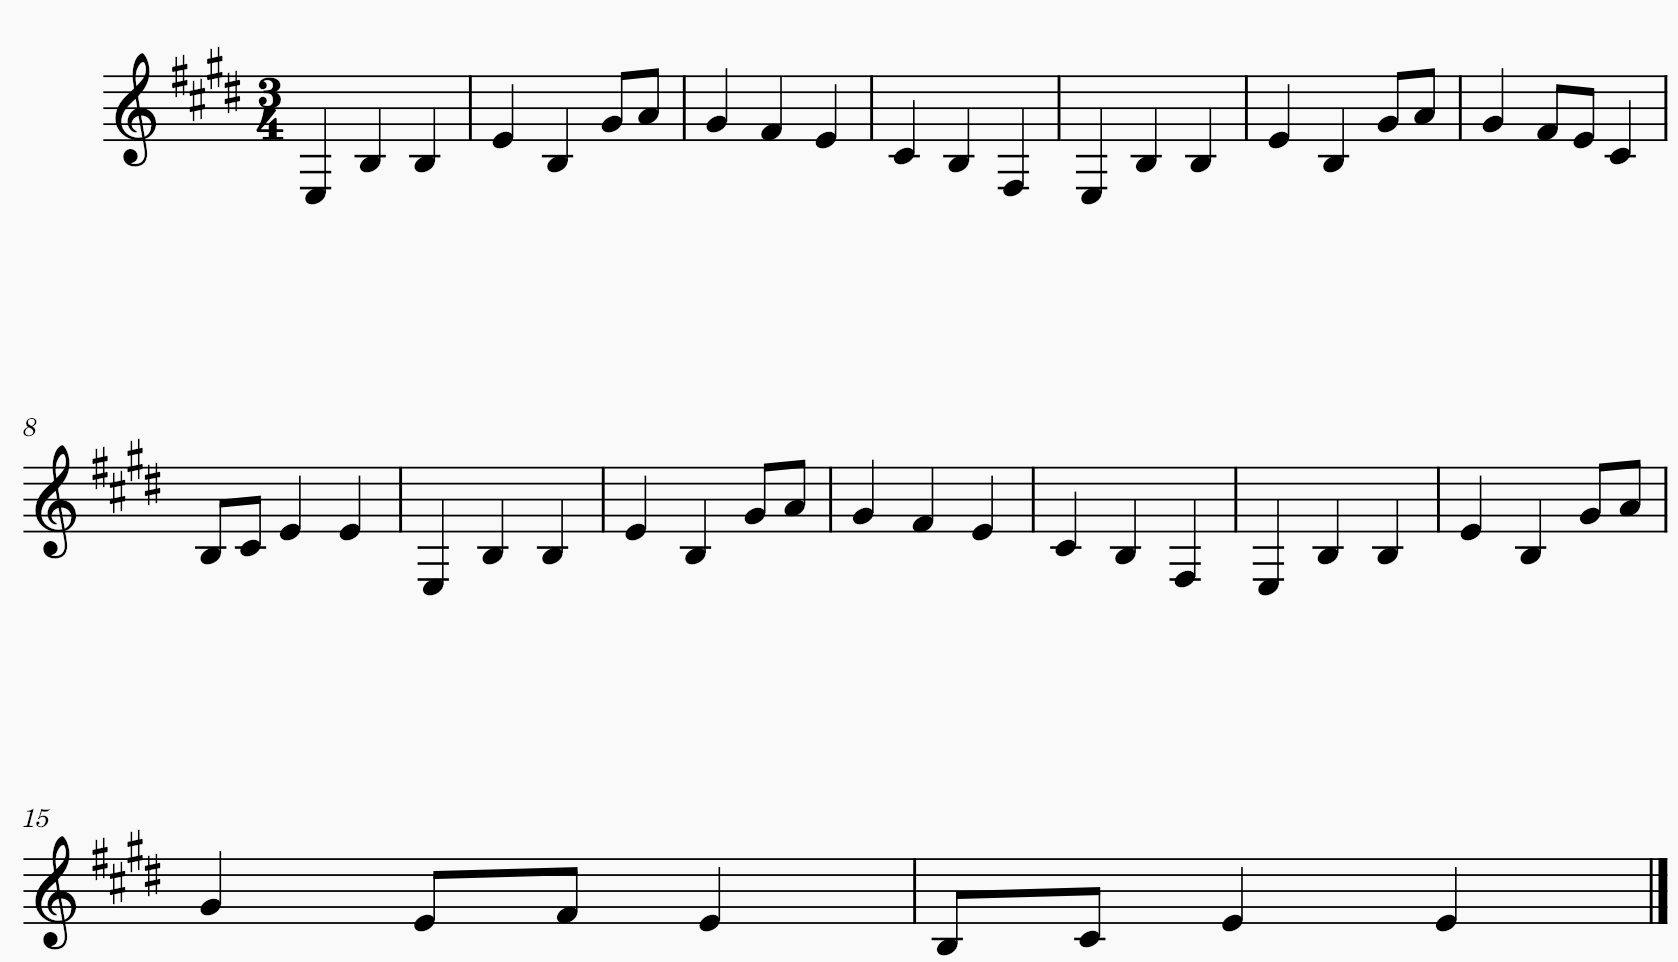
\includegraphics[width=1.0\linewidth]{images/Pink-main.png}
    \caption{主旋律}
    \label{fig:enter-label}
\end{figure}
\subsubsection{编曲结构}
音乐结构如图所示。
\begin{figure}[H]
    \centering
    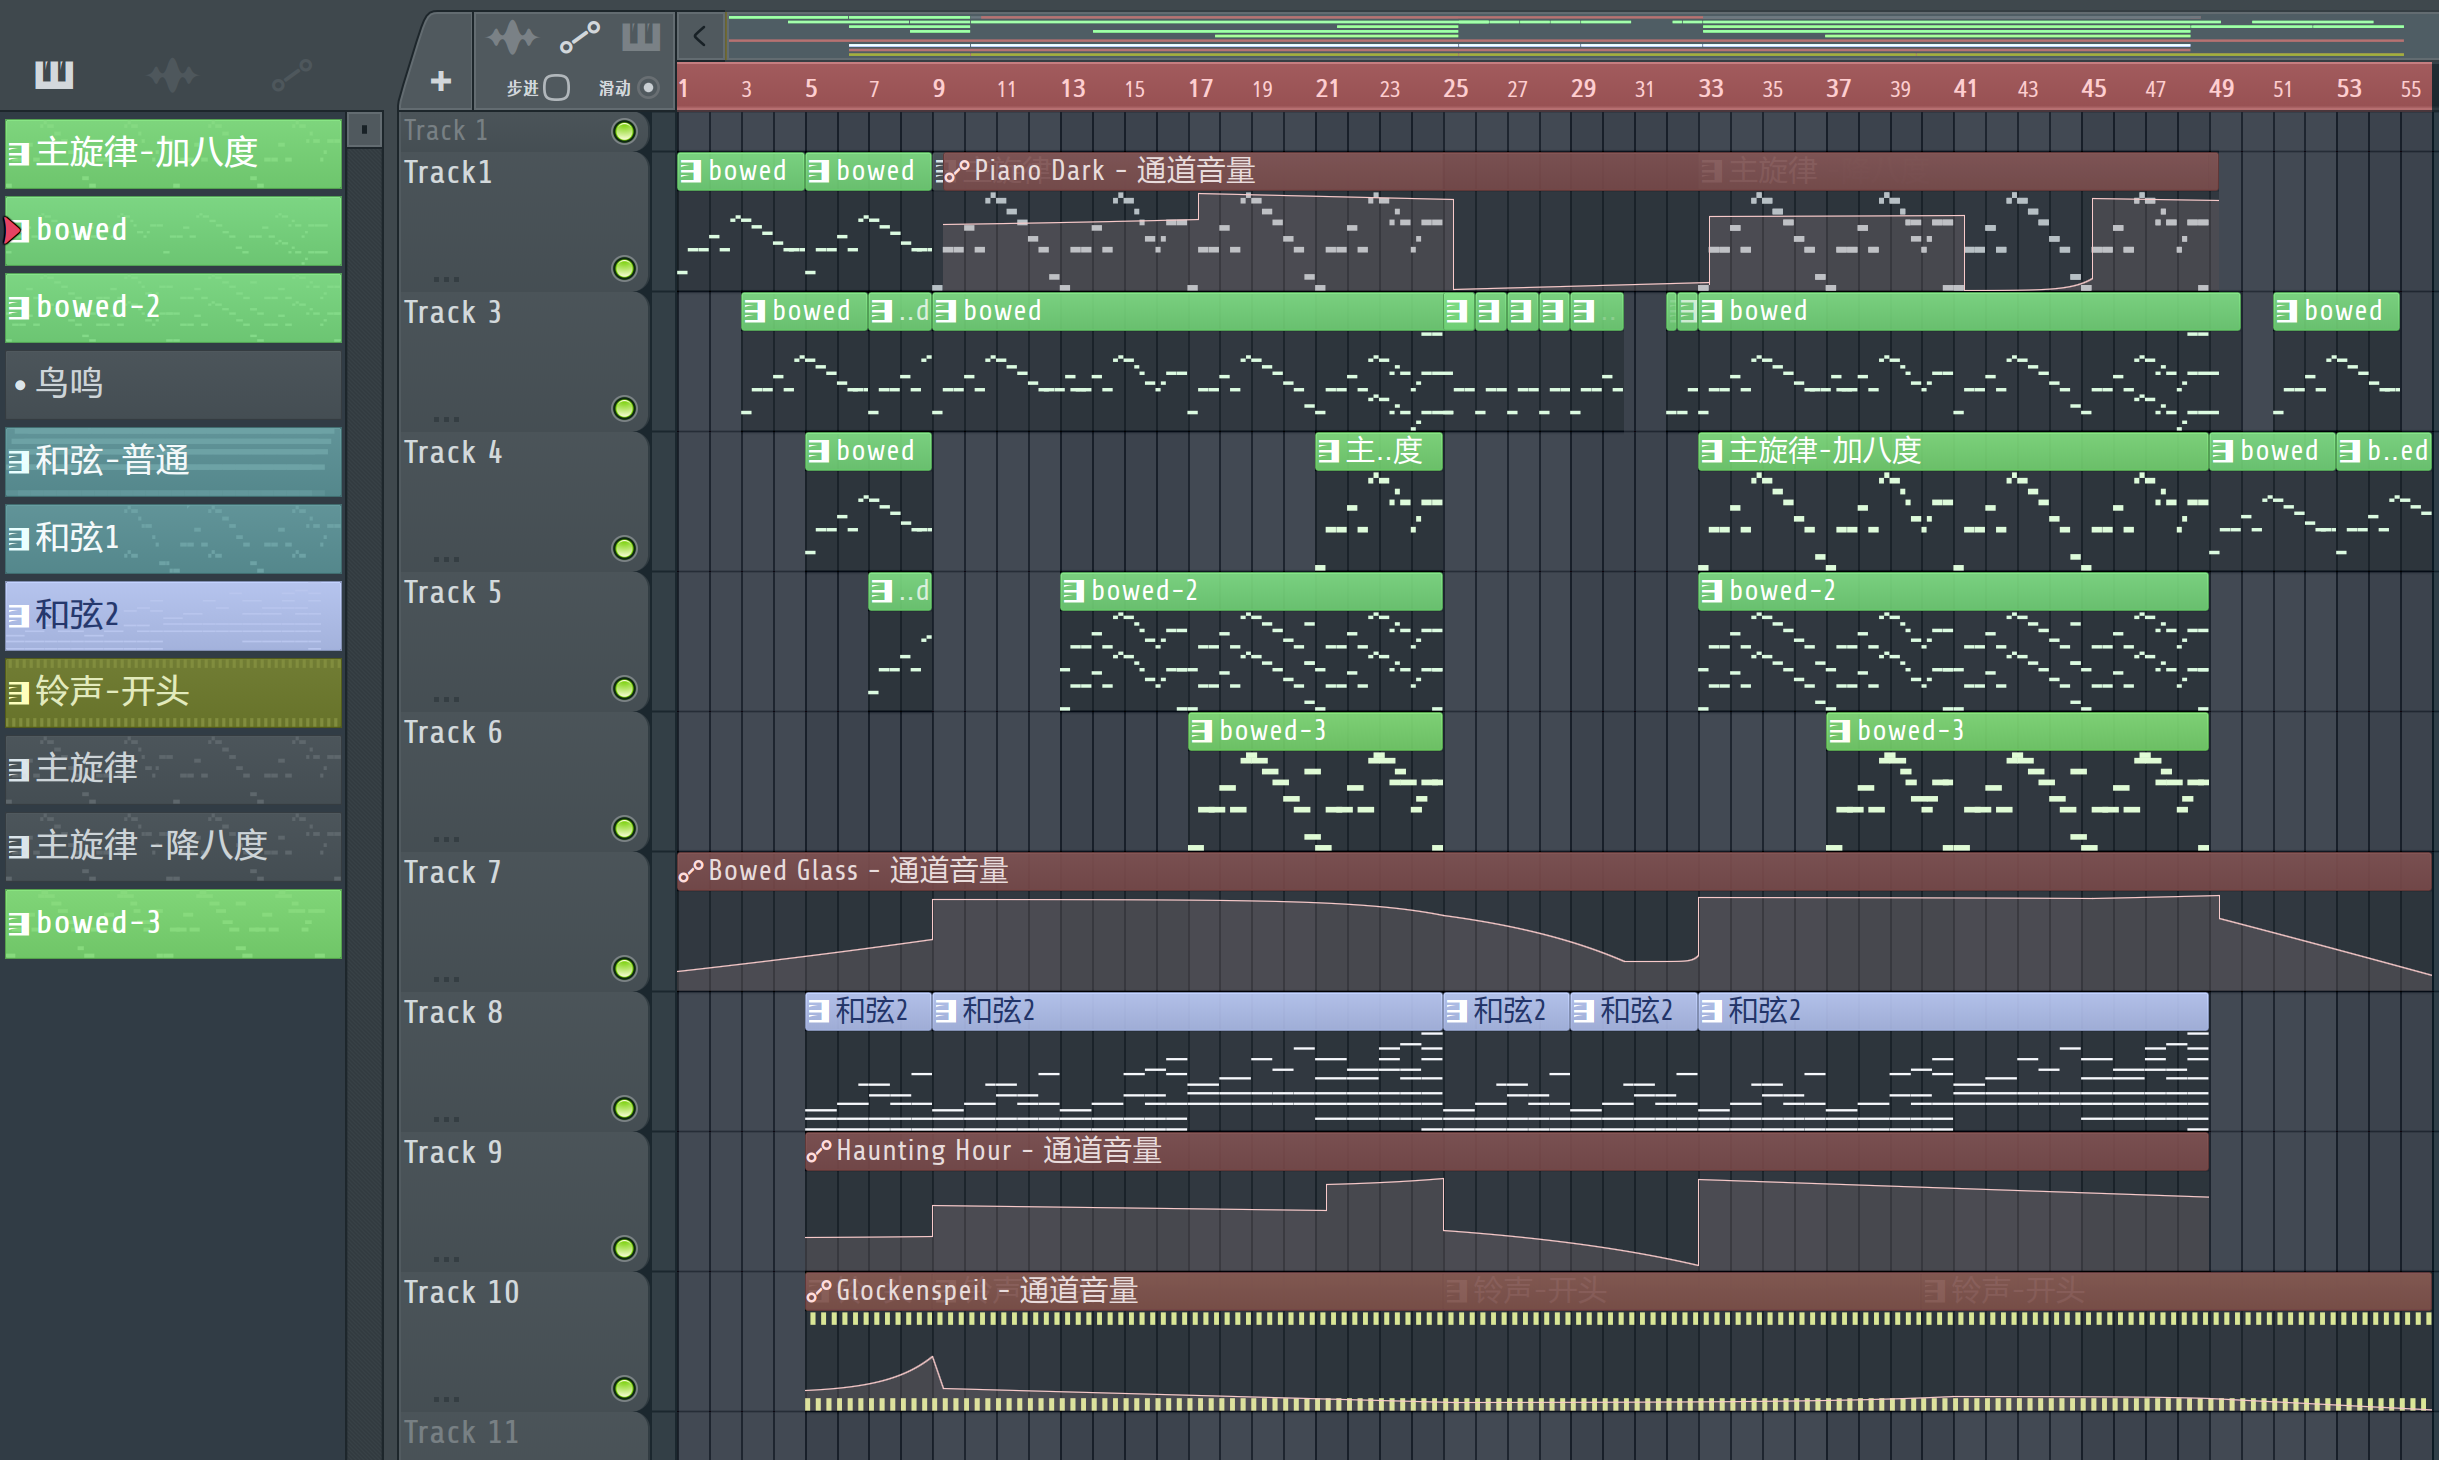
\includegraphics[width=1.0\linewidth]{images/Pink-flstudio.png}
    \caption{编曲结构}
    \label{fig:enter-label}
\end{figure}
\begin{itemize}
    \item 前奏:不断重复动机的前半部分,渐强。
    \item 第一部分:主旋律,随着旋律的推进,逐渐加入不同乐器的合奏,随后突然减弱。
    \item 第二部分:一段简单的重复,音量渐弱。
    \item 第三部分:重复主旋律,但将个别声部移高八度,并做出了一定变奏。
    \item 尾声:类似前奏的处理方式,不断重复动机的前半部分,渐弱,直到消失。
\end{itemize}


\subsubsection{乐器和音色}
我希望它给人以一种更梦幻的感受,所以主旋律使用了钢琴(Piano Dark)和吟唱的音色(FLEX - Bowed Glass)的合奏。通过调整二者的相对音量,可以实现不同的听觉效果。

和弦仍然使用Haunting Hour。

没有使用鼓点,而是使用重复的铃声(FLEX - Glockenspeil)来实现类似节拍器的效果。

\subsection{编曲的总结}

编曲的最大难点其实在于第一步,即找到随机音乐中可用的旋律片段。
由于乐谱是随机生成的,大多数片段很难被称为“悦耳动听”(就大众听感而言)。
当然,只要生成的量足够多,总能找到合适的旋律。所以我们进行了很多次Reroll,最终选择了大家都比较喜欢的片段。

(另:事后和负责代码的同学进行了交流,对方提到可以通过修改音乐生成的部分参数,来生成更“悦耳”的音乐。例如,假设我们降低时值发生变化的概率,则音乐听起来会更“均匀”一些。)

经过组内讨论,我们的目标是呈现出网易云爆款(划掉)比较符合大众喜好的纯音乐。

关于编曲结构,扒了很多纯音乐之后,发现最常见的结构是单一旋律循环。在此基础上,不断加入变奏、更换音色,就能呈现出丰富的层次感。因此编曲方式上也对此做了模仿。

最后是细节上的完善,例如全曲响度的调节,(渐强渐弱等),鸟鸣、铃声一类的音效,对音色细节的处理等。

% -----------------------------------Appendix----------------------------------------
% \appendix
\section{总结}
本次大作业的分工如下:
\begin{itemize}
    \item 音乐生成:乔天硕、赵亮然
    \item 乐谱分析:邹灵萱
    \item 编曲:张龄心
    \item 报告编写:冯之乐
\end{itemize}

我们生成音乐所使用的代码,生成的棕色音乐、粉色音乐音频,编曲的FL Studio源文件以及编曲后得到的乐曲音频均附在压缩包中,也可以从 GitHub 上获得(\href{https://github.com/lindseyzh/Music-and-Mathematics}{GitHub链接})。

% \newpage
% -----------------------------------REFERENCE----------------------------------------
\begin{thebibliography}{9}
% \bibitem{Erdos01} P. Erd\H os, \emph{A selection of problems and
% results in combinatorics}, Recent trends in combinatorics (Matrahaza,
% 1995), Cambridge Univ. Press, Cambridge, 2001, pp. 1--6.
\bibitem{book01} 李重光,\emph{基本乐理通用教材},高等教育出版社,2004.

\bibitem{book02} Martin Gardener,\emph{Fractal music, hypercards and more},W.H.Freeman and Company,1992.

\end{thebibliography}
\end{document}

